158. \begin{figure}[ht!]
\center{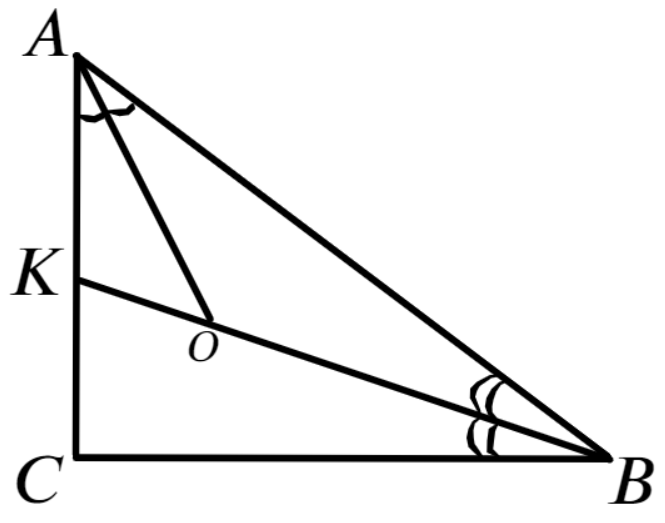
\includegraphics[scale=0.35]{g8-158.png}}
\end{figure}\\
а) По теореме Пифагора найдём $AB=\sqrt{3^2+4^2}=5.$ Посчитаем площадь двумя способами: с одной стороны, $S=\cfrac{3\cdot4}{2}=6,$ а с другой стороны $S=rp=r\cdot\cfrac{3+4+5}{2}=6r.$ Значит, $r=6:6=1.$\\
б) $\angle AOB=180^\circ-\angle OAB-\angle OBA=180^\circ-\cfrac{1}{2}(\angle A+\angle B)=180^\circ-\cfrac{1}{2}\cdot90^\circ=135^\circ.$\\
в) По теореме об основании биссектрисы $\cfrac{AK}{CK}=\cfrac{AB}{CB}=\cfrac{5}{4}.$ У треугольников $BCK$ и $BAK$ общая высота $BC,$ значит $\cfrac{S_{\Delta BAK}}{S_{\Delta BCK}}=\cfrac{5}{4},\ S_{\Delta BAK}=\cfrac{5}{4}S_{\Delta BCK}$ и $S_{\Delta BCK}+\cfrac{5}{4}S_{\Delta BCK}=6,\ S_{\Delta BCK}=\cfrac{8}{3}.$\newpage\noindent
